% ============================================================================
%  BÁO CÁO THÍ NGHIỆM LAB 4 – KIỂM TRA THIẾT KẾ SỬ DỤNG TESTBENCH
%  Môn: CE213 – Thiết kế logic số
%  Công cụ: Verilog HDL, ModelSim-Altera, Quartus II
% ============================================================================
\documentclass[12pt,a4paper]{article}

% ── Packages ────────────────────────────────────────────────────────────────
\usepackage[utf8]{inputenc}
\usepackage[vietnamese]{babel}
\usepackage{amsmath, amssymb}
\usepackage{graphicx}
\usepackage{float}
\usepackage{geometry}
\usepackage{listings}
\usepackage{xcolor}
\usepackage{caption}
\usepackage{subcaption}
\usepackage{hyperref}
\usepackage{fancyhdr}
\usepackage{titlesec}
\usepackage{booktabs}
\usepackage{enumitem}

% ── Page geometry ───────────────────────────────────────────────────────────
\geometry{left=2.5cm, right=2cm, top=2.5cm, bottom=2.5cm}

% ── Header / Footer ────────────────────────────────────────────────────────
\pagestyle{fancy}
\fancyhf{}
\fancyhead[L]{\small CE213 – Thiết kế hệ thống số với HDL}
\fancyhead[R]{\small Lab 4 – Testbench \& Verification}
\fancyfoot[C]{\thepage}

% ── Code listing style ─────────────────────────────────────────────────────
\definecolor{codebg}{RGB}{248,248,248}
\definecolor{codeframe}{RGB}{200,200,200}
\definecolor{keyword}{RGB}{0,0,180}
\definecolor{comment}{RGB}{0,128,0}
\definecolor{string}{RGB}{163,21,21}

\lstdefinestyle{verilog}{
    language=Verilog,
    backgroundcolor=\color{codebg},
    frame=single,
    rulecolor=\color{codeframe},
    basicstyle=\ttfamily\footnotesize,
    keywordstyle=\color{keyword}\bfseries,
    commentstyle=\color{comment}\itshape,
    stringstyle=\color{string},
    numbers=left,
    numberstyle=\tiny\color{gray},
    numbersep=8pt,
    breaklines=true,
    breakatwhitespace=false,
    tabsize=4,
    showstringspaces=false,
    captionpos=b,
    columns=flexible,
    literate={<=}{{$\leq$}}1 {>=}{{$\geq$}}1,
}

\lstdefinestyle{log}{
    backgroundcolor=\color{codebg},
    frame=single,
    rulecolor=\color{codeframe},
    basicstyle=\ttfamily\scriptsize,
    numbers=none,
    breaklines=true,
    tabsize=4,
    showstringspaces=false,
    captionpos=b,
}

\lstdefinestyle{md}{
    backgroundcolor=\color{codebg},
    frame=single,
    rulecolor=\color{codeframe},
    basicstyle=\ttfamily\scriptsize,
    numbers=none,
    breaklines=true,
    tabsize=2,
    showstringspaces=false,
    captionpos=b,
}

% ── Graphics path ──────────────────────────────────────────────────────────
\graphicspath{{ex1/}{ex2/}{ex3/}{ex4/}{ex5/}{ex6/}}

% ── Title format ───────────────────────────────────────────────────────────
\titleformat{\section}{\large\bfseries}{\thesection.}{0.5em}{}
\titleformat{\subsection}{\normalsize\bfseries}{\thesubsection.}{0.5em}{}

% ============================================================================
\begin{document}

% ── Trang bìa ──────────────────────────────────────────────────────────────
\begin{titlepage}
\centering
\vspace*{1cm}

{\Large\textbf{TRƯỜNG ĐẠI HỌC CÔNG NGHỆ THÔNG TIN}}\\[0.3cm]
{\Large\textbf{ĐẠI HỌC QUỐC GIA THÀNH PHỐ HỒ CHÍ MINH}}\\[0.3cm]
{\large\textbf{KHOA KỸ THUẬT MÁY TÍNH}}\\[2cm]

\rule{\textwidth}{1.5pt}\\[0.5cm]
{\LARGE\bfseries BÁO CÁO THÍ NGHIỆM}\\[0.3cm]
{\Huge\bfseries Lab 4: Testbench \& Verification}\\[0.5cm]
\rule{\textwidth}{1.5pt}\\[1.5cm]

{\large Môn học: \textbf{CE213 -- Thiết kế hệ thống số với HDL}}\\[1cm]

\begin{tabular}{ll}
    \textbf{Sinh viên:}  & Võ Trọng Kiên \\
    \textbf{MSSV:}        & 23520808 \\
    \textbf{Lớp:}         & CE213.Q23 \\
    \textbf{GVHD:}        & Hồ Ngọc Diễm \\
\end{tabular}

\vfill

{\large TP. Hồ Chí Minh, \the\year}
\end{titlepage}

% ── Mục lục ────────────────────────────────────────────────────────────────
\tableofcontents
\newpage

% ============================================================================
%  GIỚI THIỆU
% ============================================================================
\section{Giới thiệu}

\subsection{Mục tiêu}
Làm quen với việc kiểm tra thiết kế bằng phương pháp viết \textbf{Testbench} và sử dụng phần mềm \textbf{ModelSim-Altera} để mô phỏng, quan sát dạng sóng, xác minh chức năng và timing của các thiết kế Verilog. Lab 4 gồm 6 bài tập từ các mạch tổ hợp (ALU) đến mạch tuần tự (counter), bộ nhớ (register file, RAM) và cuối cùng là thực hành sử dụng chip SRAM ngoài trên kit DE2.

\subsection{Cấu trúc thư mục dự án}

\begin{lstlisting}[style=md, caption={Tổ chức thư mục \texttt{lab4/src/}}]
lab4/
  README.md                        <- hướng dẫn tổng hợp, chi tiết câu 6
  Lab4_Testbench Verification.pdf  <- đề bài
  lab8_Verilog.pdf                 <- tham khảo Part IV (SRAM DE2)
  Thuc hanh su dung IP cores.pdf   <- tham khảo Phần 4
  src/
    ex1/  alu32.v, tb_alu32.v
    ex2/  counter4.v, tb_counter4_wave.v, tb_counter4_self.v
    ex3/  reg_file_32x32.v, tb_reg_file_32x32.v
    ex4/  dual_port_ram_1kx8.v, tb_dual_port_ram_1kx8.v
    ex5/  sp_ram_128x8.v, tb_sp_ram_128x8_wave.v, tb_sp_ram_128x8_self.v
    ex6/  sram_de2_32x8.v, hex_to_7seg.v, sram_model.v, tb_sram_de2_32x8.v
\end{lstlisting}

\subsection{Phương pháp kiểm tra}
Toàn bộ testbench được xây dựng theo hai mô hình đã yêu cầu trong đề bài:

\begin{itemize}[leftmargin=1.5cm]
    \item \textbf{Mô hình quan sát dạng sóng} (câu 2.1, 5.1): chỉ phát stimulus, dump VCD và dùng \texttt{\$monitor} in giá trị các tín hiệu ra cửa sổ Transcript để kiểm tra trực quan bằng Wave window của ModelSim.
    \item \textbf{Mô hình self-checking} (câu 1, 2.2, 3, 4, 5.2, 6): duy trì một \textbf{golden model} song song với DUT, so sánh ngõ ra thực tế với giá trị kỳ vọng sau mỗi chu kỳ clock; đếm pass/fail, in kết quả PASS/FAIL kèm tag mô tả; ghi đồng thời ra stdout và file \texttt{.log}; có watchdog timeout để chặn simulation chạy vô hạn.
\end{itemize}

Các testbench đều sử dụng chung một pattern: task \texttt{tb\_log}, \texttt{tb\_section} để gom nhóm test case và ghi log có dấu thời gian; task \texttt{apply\_reset} (khi cần) để đưa DUT về trạng thái biết trước; và cuối cùng in dòng \texttt{SUMMARY} + \texttt{RESULT} tóm tắt tổng số test, số pass và số fail.

\newpage

% ============================================================================
%  EXERCISE 1: ALU 32-BIT
% ============================================================================
\section{Exercise 1: ALU 32-bit}

\subsection{Yêu cầu bài tập}
Thiết kế bộ ALU 32-bit có 3 tín hiệu điều khiển $\{M, S_1, S_0\}$ thực hiện 8 phép toán theo bảng sau; viết testbench tạo giá trị cho input và quan sát kết quả bằng các thủ tục \texttt{\$display} và \texttt{\$monitor}, chạy mô phỏng kiểm tra chức năng và timing bằng ModelSim-Altera.

\begin{table}[H]
\centering
\begin{tabular}{ccc|l|l}
\toprule
$M$ & $S_1$ & $S_0$ & \textbf{Phép toán} & \textbf{Mô tả} \\
\midrule
0 & 0 & 0 & $Y = \sim A$       & Complement A \\
0 & 0 & 1 & $Y = A \ \&\  B$   & AND \\
0 & 1 & 0 & $Y = A \oplus B$   & EX-OR \\
0 & 1 & 1 & $Y = A \mid B$     & OR \\
1 & 0 & 0 & $Y = A - 1$        & Decrement A \\
1 & 0 & 1 & $Y = A + B$        & Add \\
1 & 1 & 0 & $Y = A - B$        & Subtract \\
1 & 1 & 1 & $Y = A + 1$        & Increment A \\
\bottomrule
\end{tabular}
\caption{Bảng chức năng ALU 32-bit}
\end{table}

% ── Source code ────────────────────────────────────────────────────────────
\subsection{Mã nguồn Verilog}

\subsubsection{DUT: \texttt{alu32.v}}
\lstinputlisting[style=verilog, caption={alu32.v}]{ex1/alu32.v}

\textbf{Giải thích:} DUT dùng một khối \texttt{always @(*)} kết hợp \texttt{case(\{M,S1,S0\})} để giải mã 8 op-code. Toàn bộ là tổ hợp (không có thanh ghi) nên thay đổi tín hiệu điều khiển hoặc toán hạng sẽ cập nhật $Y$ ngay lập tức. Mẫu \texttt{default} gán \texttt{32'hxxxx\_xxxx} giúp dễ phát hiện lỗi giải mã trong mô phỏng.

\subsubsection{Testbench: \texttt{tb\_alu32.v}}
\lstinputlisting[style=verilog, caption={tb\_alu32.v}]{ex1/tb_alu32.v}

\textbf{Giải thích:}
\begin{itemize}[leftmargin=1.5cm]
    \item Dùng \texttt{\$monitor} in header mỗi khi tín hiệu đổi; dùng \texttt{\$display} in kết quả PASS/FAIL theo yêu cầu đề.
    \item Hàm \texttt{expected(op, a, b)} tính giá trị kỳ vọng bằng chính biểu thức Verilog tương đương $\rightarrow$ làm golden model.
    \item Hai bộ test: \texttt{run\_all\_ops()} chạy mỗi op-code với 2 cặp $(A,B)$ (một trực quan $0x0F/0xF0$, một biên $0xFFFFFFFF/0x00000001$ để kiểm tra tràn/mượn); \texttt{run\_random\_ops()} chạy thêm 16 op-code ngẫu nhiên.
    \item Có VCD dump, log file và watchdog $5000$\,ns.
\end{itemize}

% ── Simulation results ─────────────────────────────────────────────────────
\subsection{Kết quả mô phỏng}

\subsubsection{Dạng sóng ModelSim}

\begin{figure}[H]
    \centering
    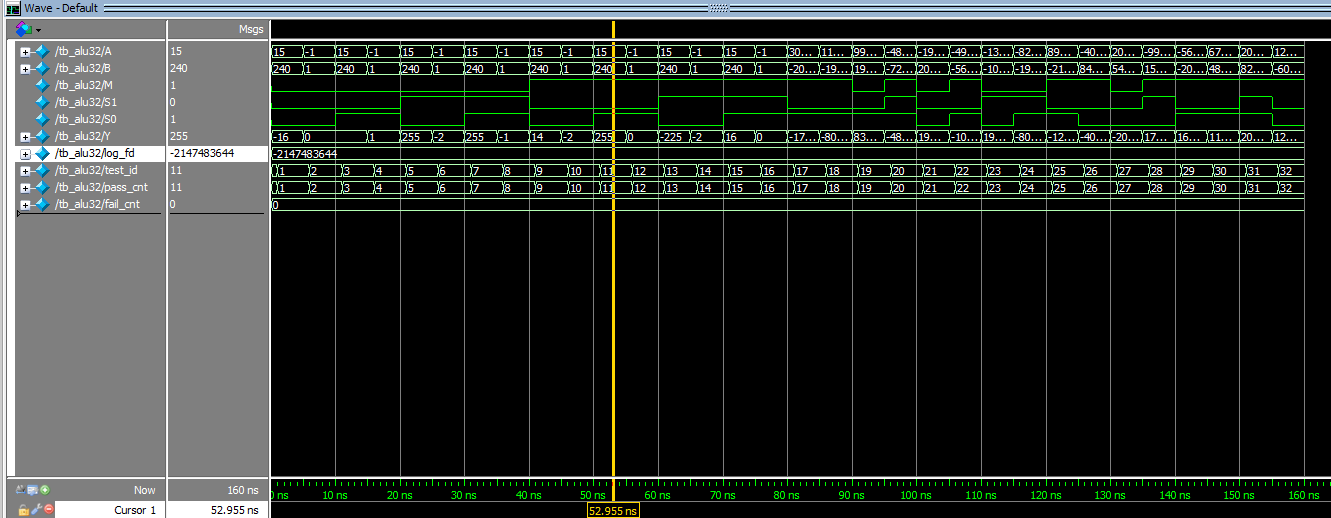
\includegraphics[width=\textwidth]{ex1/wv.png}
    \caption{Dạng sóng -- ALU 32-bit (Wave window)}
    \label{fig:ex1_wave}
\end{figure}

\begin{figure}[H]
    \centering
    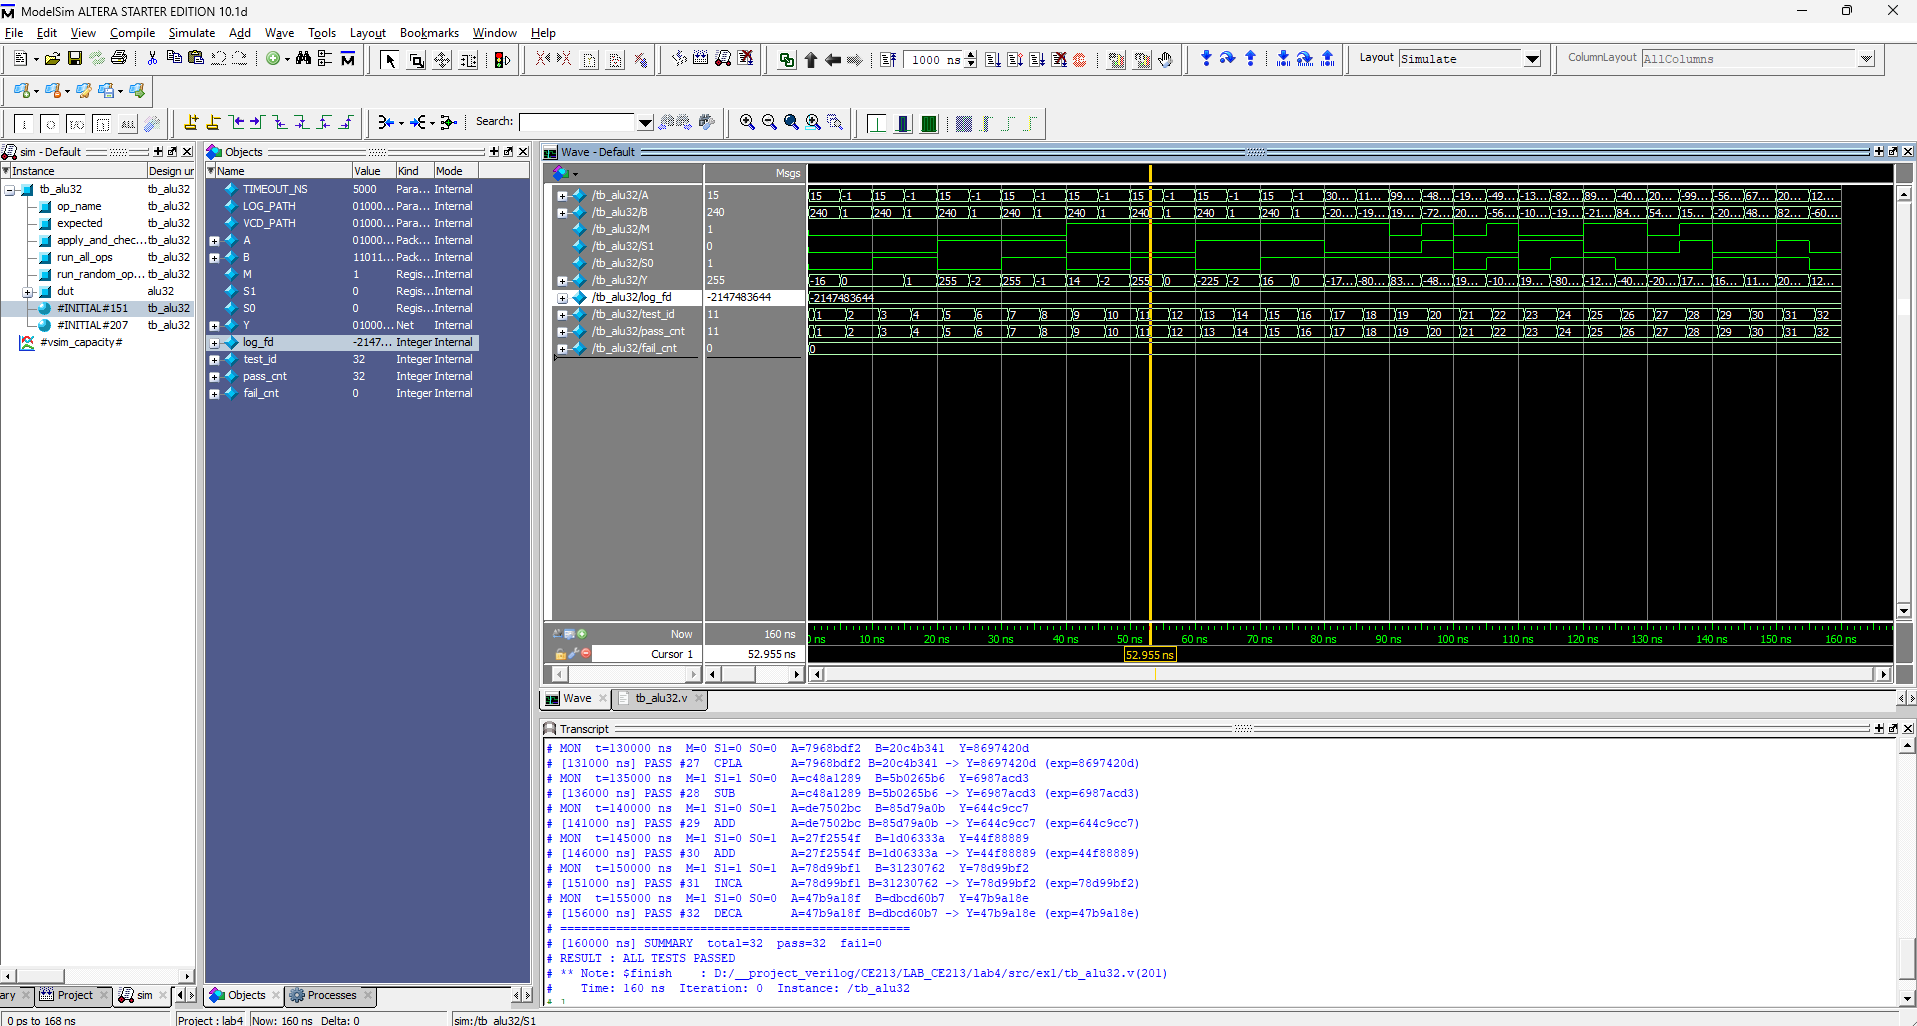
\includegraphics[width=\textwidth]{ex1/modelsim.png}
    \caption{Transcript ModelSim -- ALU 32-bit (\texttt{\$display}/\texttt{\$monitor})}
    \label{fig:ex1_transcript}
\end{figure}

\subsubsection{Tóm tắt kết quả Simulation Log}

\begin{lstlisting}[style=log, caption={Tóm tắt -- tb\_alu32.log}]
[160000 ns] SUMMARY  total=32  pass=32  fail=0
RESULT : ALL TESTS PASSED
\end{lstlisting}

Toàn bộ 32 test case (16 cặp cố định cho 8 op-code + 16 op-code ngẫu nhiên) đều \textbf{PASS}. ALU giải mã và tính toán đúng cho cả trường hợp biên (tràn add, mượn sub).

\newpage

% ============================================================================
%  EXERCISE 2: COUNTER 4-BIT
% ============================================================================
\section{Exercise 2: Counter 4-bit}

\subsection{Yêu cầu bài tập}
Thiết kế bộ đếm 4-bit với các tín hiệu:
\begin{itemize}[leftmargin=1.5cm]
    \item \texttt{clock}: kích cạnh lên.
    \item \texttt{reset\_n}: bất đồng bộ, tích cực thấp.
    \item \texttt{enable}: cho phép đếm (tích cực cao).
    \item \texttt{up\_down}: điều khiển hướng đếm ($0$ = đếm lên, $1$ = đếm xuống).
\end{itemize}

Yêu cầu viết \textbf{hai} testbench: (2.1) mô hình quan sát dạng sóng, (2.2) mô hình tự kiểm tra (self-checking).

\subsection{Mã nguồn Verilog}

\subsubsection{DUT: \texttt{counter4.v}}
\lstinputlisting[style=verilog, caption={counter4.v}]{ex2/counter4.v}

\textbf{Giải thích:} Một khối \texttt{always @(posedge clock or negedge reset\_n)}. Khi \texttt{reset\_n = 0} (bất đồng bộ), \texttt{q\_out} về 0. Khi \texttt{enable = 1}, \texttt{q\_out} được cộng/trừ 1 tuỳ \texttt{up\_down}; khi \texttt{enable = 0} giữ nguyên giá trị cũ.

\subsection{Câu 2.1 -- Mô hình quan sát dạng sóng}

\subsubsection{Testbench: \texttt{tb\_counter4\_wave.v}}
\lstinputlisting[style=verilog, caption={tb\_counter4\_wave.v}]{ex2/tb_counter4_wave.v}

\textbf{Giải thích:} Phát kịch bản stimulus gồm reset, đếm lên 20 chu kỳ (bao phủ rollover $F\to 0$), tắt \texttt{enable} giữ 5 chu kỳ, đếm xuống 20 chu kỳ (rollover $0\to F$) và cuối cùng là async reset giữa chu kỳ. Không tự kiểm tra, chỉ dump VCD và \texttt{\$monitor} để quan sát.

\subsubsection{Kết quả dạng sóng}
\begin{figure}[H]
    \centering
    
\includegraphics[width=\textwidth]{ex2/wv.png}
    \caption{Dạng sóng -- Counter 4-bit (testbench wave)}
    \label{fig:ex2_wave}
\end{figure}

Có thể quan sát rõ: \texttt{q\_out} đếm $0{\to}F$ khi \texttt{up\_down=0}, giữ nguyên khi \texttt{enable=0}, chuyển sang đếm xuống khi \texttt{up\_down=1}, và về 0 tức thời ở thời điểm \texttt{reset\_n} xuống thấp.

\subsection{Câu 2.2 -- Mô hình self-checking}

\subsubsection{Testbench: \texttt{tb\_counter4\_self.v}}
\lstinputlisting[style=verilog, caption={tb\_counter4\_self.v}]{ex2/tb_counter4_self.v}

\textbf{Giải thích:}
\begin{itemize}[leftmargin=1.5cm]
    \item Duy trì \texttt{reg [3:0] exp\_q} làm golden model, cập nhật theo cùng quy luật với DUT trong task \texttt{update\_golden}.
    \item Task \texttt{tick\_and\_check} chờ cạnh lên clock, update golden, sau \texttt{\#1} so sánh \texttt{q\_out === exp\_q} và đếm pass/fail.
    \item 5 test case: đếm lên 20 chu kỳ (rollover), \texttt{enable=0} giữ giá trị, đếm xuống 20 chu kỳ (rollover), bật-tắt enable xen kẽ, async reset giữa chu kỳ.
\end{itemize}

\subsubsection{Kết quả self-check}
\begin{figure}[H]
    \centering
    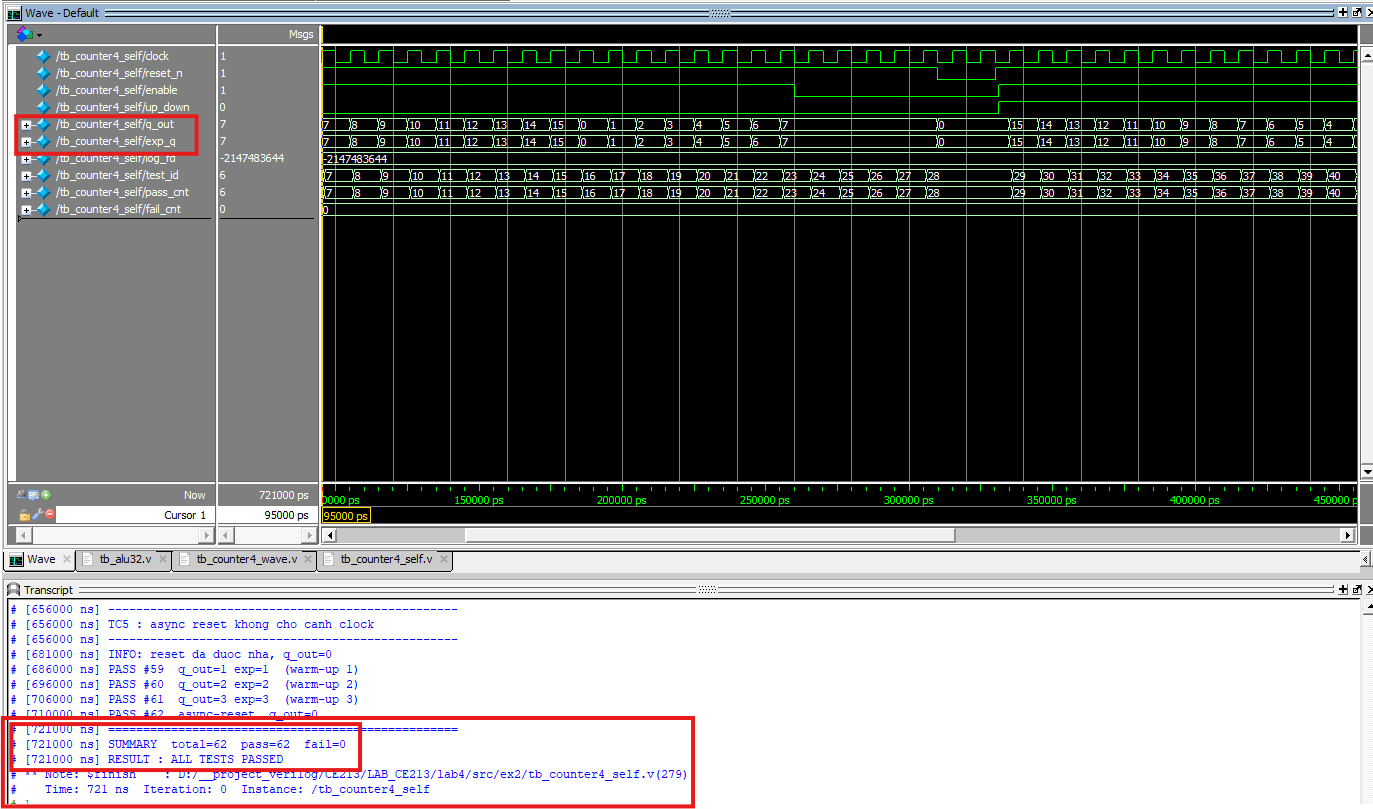
\includegraphics[width=\textwidth]{ex2/self_check.png}
    \caption{Transcript ModelSim -- Counter 4-bit self-checking}
    \label{fig:ex2_self}
\end{figure}

\begin{lstlisting}[style=log, caption={Tóm tắt -- tb\_counter4\_self.log}]
[721000 ns] SUMMARY  total=62  pass=62  fail=0
[721000 ns] RESULT : ALL TESTS PASSED
\end{lstlisting}

Toàn bộ 62 check (tương ứng 20+5+20+10+7 chu kỳ kiểm tra) đều \textbf{PASS}: counter đếm lên, đếm xuống, rollover ở cả hai chiều, giữ giá trị khi \texttt{enable=0} và reset bất đồng bộ đều chính xác.

\newpage

% ============================================================================
%  EXERCISE 3: REGISTER FILE 32x32
% ============================================================================
\section{Exercise 3: Register File 32$\times$32}

\subsection{Yêu cầu bài tập}
Thiết kế tập thanh ghi gồm \textbf{32 thanh ghi, mỗi thanh ghi 4 byte (32-bit)} với \textbf{2 port đọc, 1 port ghi}. Các tín hiệu: \texttt{ReadAddress1[4:0]}, \texttt{ReadAddress2[4:0]}, \texttt{WriteAddress[4:0]}, \texttt{WriteData[31:0]}, \texttt{ReadData1[31:0]}, \texttt{ReadData2[31:0]}, \texttt{WriteEn}.

\subsection{Mã nguồn Verilog}

\subsubsection{DUT: \texttt{reg\_file\_32x32.v}}
\lstinputlisting[style=verilog, caption={reg\_file\_32x32.v}]{ex3/reg_file_32x32.v}

\textbf{Giải thích:} Tập thanh ghi được khai báo dưới dạng mảng \texttt{reg [31:0] regs[0:31]}. Ghi đồng bộ ở cạnh lên \texttt{clk} khi \texttt{WriteEn=1}; đọc bất đồng bộ (combinational) trên cả 2 port -- đúng mô hình register file của MIPS. Không hard-wire R0 về 0 (theo đặc tả đề chỉ nói ``32 thanh ghi'').

\subsubsection{Testbench: \texttt{tb\_reg\_file\_32x32.v}}
\lstinputlisting[style=verilog, caption={tb\_reg\_file\_32x32.v}]{ex3/tb_reg_file_32x32.v}

\textbf{Giải thích:}
\begin{itemize}[leftmargin=1.5cm]
    \item Golden model nội bộ \texttt{reg [31:0] golden [0:31]} khởi tạo 0 và cập nhật đồng bộ với task \texttt{rf\_write}.
    \item 5 test case: ghi tuần tự 32 thanh ghi rồi đọc qua cả 2 port; read-during-write; \texttt{WriteEn=0} không thay đổi dữ liệu; 2 port đọc độc lập với 2 địa chỉ khác nhau; 50 lần ghi ngẫu nhiên bằng \texttt{\$random}.
\end{itemize}

\subsection{Kết quả self-check}

\begin{figure}[H]
    \centering
    
\includegraphics[width=\textwidth]{ex3/self_check.png}
    \caption{Transcript ModelSim -- Register File 32$\times$32}
    \label{fig:ex3_self}
\end{figure}

\begin{lstlisting}[style=log, caption={Tóm tắt -- tb\_reg\_file\_32x32.log}]
[1822000 ns] SUMMARY  total=170  pass=170  fail=0
[1822000 ns] RESULT : ALL TESTS PASSED
\end{lstlisting}

Toàn bộ 170 check đều \textbf{PASS}: ghi/đọc tuần tự 32 thanh ghi, read-during-write, gated write (WriteEn=0), dual-port đọc độc lập và 100 lần đọc ngẫu nhiên sau 50 lần ghi ngẫu nhiên đều cho kết quả đúng.

\newpage

% ============================================================================
%  EXERCISE 4: DUAL-PORT RAM 1024x8
% ============================================================================
\section{Exercise 4: Dual-port RAM 1024$\times$8}

\subsection{Yêu cầu bài tập}
Hiện thực một \textbf{dual-port RAM} kích thước $1024 \times 8$ (dung lượng 1\,KB) với các tín hiệu: \texttt{Address[9:0]}, \texttt{WriteData[7:0]}, \texttt{ReadData[7:0]}, \texttt{WriteEn}, \texttt{ReadEn}. Viết testbench tạo giá trị cho input và chạy mô phỏng kiểm tra chức năng và timing.

\subsection{Mã nguồn Verilog}

\subsubsection{DUT: \texttt{dual\_port\_ram\_1kx8.v}}
\lstinputlisting[style=verilog, caption={dual\_port\_ram\_1kx8.v}]{ex4/dual_port_ram_1kx8.v}

\textbf{Giải thích:} Vì đặc tả chỉ có một \texttt{Address}, một \texttt{WriteData}, một \texttt{ReadData} nên được hiện thực theo kiểu 1R1W trên cùng địa chỉ: sync-write khi \texttt{WriteEn=1} và gated sync-read khi \texttt{ReadEn=1}. Cấu trúc này khớp với block M4K của Cyclone II (single-clock, registered output tuỳ chọn).

\subsubsection{Testbench: \texttt{tb\_dual\_port\_ram\_1kx8.v}}
\lstinputlisting[style=verilog, caption={tb\_dual\_port\_ram\_1kx8.v}]{ex4/tb_dual_port_ram_1kx8.v}

\textbf{Giải thích:}
\begin{itemize}[leftmargin=1.5cm]
    \item Golden 1024 byte \texttt{reg [7:0] gold [0:1023]}.
    \item Task \texttt{mem\_write(addr, data)} ghi đồng bộ; task \texttt{mem\_read\_check(addr, tag)} thực hiện sync read (chờ 1 cạnh lên sau khi ReadEn=1) rồi so sánh với \texttt{gold[addr]}.
    \item 5 test case: biên \texttt{Address=0/1023}, pattern \texttt{mem[i]=i[7:0]} cho $i=0..255$, \texttt{WriteEn=0} không đổi RAM, \texttt{ReadEn=0} giữ \texttt{ReadData} cũ (gated read), 100 giao dịch ngẫu nhiên.
\end{itemize}

\subsection{Kết quả self-check}

\begin{figure}[H]
    \centering
    
\includegraphics[width=\textwidth]{ex4/self_check.png}
    \caption{Transcript ModelSim -- Dual-port RAM 1024$\times$8}
    \label{fig:ex4_self}
\end{figure}

\begin{lstlisting}[style=log, caption={Tóm tắt -- tb\_dual\_port\_ram\_1kx8.log}]
[14480000 ns] SUMMARY  total=362  pass=362  fail=0
[14480000 ns] RESULT : ALL TESTS PASSED
\end{lstlisting}

Toàn bộ 362 check (2 biên $\times$ 2 + 256 pattern read + 2 ghi-tắt + 1 gated read + 100 random write + 100 random read $\approx$ 362) đều \textbf{PASS}. RAM hoạt động đúng ở cả chế độ gated read, gated write, và 100 giao dịch ngẫu nhiên xuyên suốt 1024 địa chỉ.

\newpage

% ============================================================================
%  EXERCISE 5: SINGLE-PORT SYNC RAM 128x8 (INOUT)
% ============================================================================
\section{Exercise 5: Single-port Sync RAM 128$\times$8 (bus \texttt{inout})}

\subsection{Yêu cầu bài tập}
Thiết kế \textbf{single-port RAM đồng bộ read/write} kích thước $128 \times 8$ với tín hiệu:
\begin{itemize}[leftmargin=1.5cm]
    \item \texttt{clock}: kích cạnh lên.
    \item \texttt{cs}: chip-select.
    \item \texttt{wr\_e}: $1$ = ghi, $0$ = đọc.
    \item \texttt{oe}: output enable.
    \item \texttt{addr[6:0]}: địa chỉ (128 byte).
    \item \texttt{data[7:0]}: \textbf{kiểu inout}.
\end{itemize}

Viết hai testbench: (5.1) mô hình quan sát dạng sóng, (5.2) mô hình self-checking.

\subsection{Mã nguồn Verilog}

\subsubsection{DUT: \texttt{sp\_ram\_128x8.v}}
\lstinputlisting[style=verilog, caption={sp\_ram\_128x8.v}]{ex5/sp_ram_128x8.v}

\textbf{Giải thích:} Hai khối \texttt{always @(posedge clock)} xử lý riêng ghi và đọc. Register \texttt{rdata} lưu giá trị đọc ra. Lệnh \texttt{assign data = (cs \&\& !wr\_e \&\& oe) ? rdata : 8'bz} biến \texttt{data} thành tri-state: chỉ drive khi DUT đang ở chế độ đọc và \texttt{oe=1}, còn lại thả Z để cho thiết bị ngoài drive bus.

\subsection{Câu 5.1 -- Mô hình quan sát dạng sóng}

\subsubsection{Testbench: \texttt{tb\_sp\_ram\_128x8\_wave.v}}
\lstinputlisting[style=verilog, caption={tb\_sp\_ram\_128x8\_wave.v}]{ex5/tb_sp_ram_128x8_wave.v}

\textbf{Giải thích:} Tb dùng \texttt{reg [7:0] drv\_data} kết hợp \texttt{assign data = (cs \&\& wr\_e) ? drv\_data : 8'bz} để drive bus inout khi ghi và thả Z khi đọc. Kịch bản: ghi 4 địa chỉ (0, 1, 63, 127) rồi đọc lại, sau đó chuyển qua \texttt{cs=0}, \texttt{oe=0} để quan sát \texttt{data=Z}.

\begin{figure}[H]
    \centering
    
\includegraphics[width=\textwidth]{ex5/wv.png}
    \caption{Dạng sóng -- Single-port RAM 128$\times$8, bus inout}
    \label{fig:ex5_wave}
\end{figure}

\subsection{Câu 5.2 -- Mô hình self-checking}

\subsubsection{Testbench: \texttt{tb\_sp\_ram\_128x8\_self.v}}
\lstinputlisting[style=verilog, caption={tb\_sp\_ram\_128x8\_self.v}]{ex5/tb_sp_ram_128x8_self.v}

\textbf{Giải thích:}
\begin{itemize}[leftmargin=1.5cm]
    \item Cơ chế drive bus: giống TB wave (\texttt{drv\_data} + tri-state).
    \item Task \texttt{ram\_write} / \texttt{ram\_read\_check} quản lý toàn bộ chu kỳ truy cập (set \texttt{cs/wr\_e/oe/addr}, wait posedge, check, deassert).
    \item Task \texttt{expect\_high\_z} kiểm tra bus phải là \texttt{Z} khi DUT không drive.
    \item 5 test case: ghi/đọc 128 byte \texttt{mem[i] = i \^{} 0xA5}, \texttt{cs=0} khi ghi không đổi RAM, \texttt{oe=0} hoặc \texttt{cs=0} $\to$ bus $Z$, back-to-back ghi+đọc, 50 giao dịch ngẫu nhiên.
\end{itemize}

\begin{figure}[H]
    \centering
    
\includegraphics[width=\textwidth]{ex5/self_check.png}
    \caption{Transcript ModelSim -- Single-port RAM 128$\times$8 self-checking}
    \label{fig:ex5_self}
\end{figure}

\begin{lstlisting}[style=log, caption={Tóm tắt -- tb\_sp\_ram\_128x8\_self.log}]
[7280000 ns] SUMMARY  total=183  pass=183  fail=0
[7280000 ns] RESULT : ALL TESTS PASSED
\end{lstlisting}

Toàn bộ 183 check đều \textbf{PASS}. DUT ghi/đọc đúng 128 byte, bus \texttt{data} tri-state chính xác khi \texttt{cs=0} hoặc \texttt{oe=0}, và xử lý đúng 50 giao dịch ngẫu nhiên.

\newpage

% ============================================================================
%  EXERCISE 6: EXTERNAL SRAM ON DE2 BOARD
% ============================================================================
\section{Exercise 6: Thực hành sử dụng chip SRAM trên board DE2}

\subsection{Yêu cầu bài tập}
Thực hành sử dụng chip SRAM có sẵn trên board DE2 (\texttt{IS61LV25616AL-10}) để hiện thực bộ nhớ $32 \times 8$ và kiểm tra quá trình đọc/ghi trên chip, theo hướng dẫn Lab8\_Verilog Part IV và ``Thực hành sử dụng IP cores'' Phần 4.

\subsection{Đặc điểm phần cứng chip SRAM trên DE2}

Chip \texttt{IS61LV25616AL-10} có dung lượng $256\text{K} \times 16$-bit với bus địa chỉ 18-bit \texttt{A[17:0]} và bus dữ liệu hai chiều 16-bit \texttt{I/O[15:0]}. Năm chân điều khiển đều tích cực thấp:

\begin{table}[H]
\centering
\begin{tabular}{l|l|l}
\toprule
\textbf{Chân SRAM} & \textbf{Ý nghĩa} & \textbf{Tên pin DE2} \\
\midrule
\texttt{/CE} & Chip Enable & \texttt{SRAM\_CE\_N} \\
\texttt{/OE} & Output Enable & \texttt{SRAM\_OE\_N} \\
\texttt{/WE} & Write Enable & \texttt{SRAM\_WE\_N} \\
\texttt{/UB} & Upper Byte Enable & \texttt{SRAM\_UB\_N} \\
\texttt{/LB} & Lower Byte Enable & \texttt{SRAM\_LB\_N} \\
\texttt{A[17:0]}  & Address bus & \texttt{SRAM\_ADDR[17:0]} \\
\texttt{I/O[15:0]}& Data bus (inout) & \texttt{SRAM\_DQ[15:0]} \\
\bottomrule
\end{tabular}
\caption{Bảng pin DE2 $\leftrightarrow$ chip SRAM (Lab8 Part IV, Table 3)}
\end{table}

Theo khuyến nghị Lab8 Part IV, sử dụng chế độ đơn giản: tie $\overline{CE}=\overline{OE}=\overline{UB}=\overline{LB}=0$ và chỉ điều khiển bằng $\overline{WE}$. Timing chính: $t_{AA} \leq 10$\,ns (address access), $t_{AW} \geq 8$\,ns (address setup), $t_{SD} \geq 6$\,ns (data setup).

\subsection{Mã nguồn Verilog}

\subsubsection{Top-level: \texttt{sram\_de2\_32x8.v}}
\lstinputlisting[style=verilog, caption={sram\_de2\_32x8.v}]{ex6/sram_de2_32x8.v}

\textbf{Giải thích:}
\begin{itemize}[leftmargin=1.5cm]
    \item Ánh xạ user I/O: \texttt{SW[7:0]} = data-in, \texttt{SW[15:11]} = 5-bit address, \texttt{SW[17]} = Write; \texttt{KEY[0]} = clock; \texttt{HEX7,HEX6} hiển thị địa chỉ; \texttt{HEX5,HEX4} hiển thị data-in; \texttt{HEX1,HEX0} hiển thị data-out; \texttt{LEDG[0]} báo chế độ Write.
    \item Điều khiển SRAM: \texttt{CE\_N=OE\_N=UB\_N=LB\_N=0} (tie cứng), \texttt{WE\_N = \~write\_en}, địa chỉ $\texttt{SRAM\_ADDR}=\{\texttt{13'b0}, \texttt{addr\_5b}\}$.
    \item Bus inout \texttt{SRAM\_DQ}: khi ghi DUT drive $\{\texttt{8'b0}, \texttt{data\_in}\}$; khi đọc thả \texttt{16'bz} để chip SRAM drive bus; 8 bit thấp được lấy làm \texttt{data\_out}.
\end{itemize}

\subsubsection{Module phụ: \texttt{hex\_to\_7seg.v}}
\lstinputlisting[style=verilog, caption={hex\_to\_7seg.v}]{ex6/hex_to_7seg.v}

\subsubsection{Mô hình behavioral chip SRAM: \texttt{sram\_model.v}}
\lstinputlisting[style=verilog, caption={sram\_model.v -- chỉ dùng trong mô phỏng}]{ex6/sram_model.v}

\textbf{Lưu ý:} Module này \textbf{không phải RTL synthesize được}, nó thay thế chip SRAM thực tế khi chạy ModelSim để kiểm tra logic của top-level. Ghi được trigger ở cạnh xuống của \texttt{WE\_N} khớp với datasheet của \texttt{IS61LV25616AL}; đọc là combinational theo \texttt{A} khi \texttt{CE\_N=OE\_N=0} và byte-enable tương ứng bằng 0.

\subsubsection{Testbench: \texttt{tb\_sram\_de2\_32x8.v}}
\lstinputlisting[style=verilog, caption={tb\_sram\_de2\_32x8.v}]{ex6/tb_sram_de2_32x8.v}

\textbf{Giải thích:}
\begin{itemize}[leftmargin=1.5cm]
    \item Testbench nối \texttt{sram\_de2\_32x8} (DUT top-level) với \texttt{sram\_model} (thay chip SRAM ngoài).
    \item Task \texttt{do\_write(addr, data)} mô phỏng thao tác người dùng: đặt Write=1, chỉnh \texttt{SW}, nhấn--nhả \texttt{KEY[0]}, nhả Write về 0 để latch dữ liệu vào SRAM.
    \item Task \texttt{do\_read\_check(addr, expected)}: đặt Write=0, chỉnh \texttt{SW[15:11]}, chờ bus ổn định, dùng hàm \texttt{seg\_to\_hex} giải mã ngược 7-segment từ \texttt{HEX1}/\texttt{HEX0} để lấy giá trị hiển thị trên board, so sánh với expected.
    \item 2 test case: ghi 32 ô nhớ pattern \texttt{i \^{} 0xA5} rồi đọc lại; ghi/đọc biên \texttt{addr=0, 31}.
\end{itemize}

\subsection{Kết quả mô phỏng}

\begin{lstlisting}[style=log, caption={Tóm tắt -- tb\_sram\_de2\_32x8.log}]
[1360000 ns] SUMMARY  total=34  pass=34  fail=0
[1360000 ns] RESULT : ALL TESTS PASSED
\end{lstlisting}

Toàn bộ 34 check (32 ô nhớ + 2 biên) đều \textbf{PASS} trong mô phỏng: top-level kết nối SRAM ngoài đúng giao thức đọc/ghi, bus inout hoạt động chính xác, 7-segment hiển thị đúng giá trị đã ghi.

\subsection{Nạp kit và kiểm tra trên board DE2}

Sau khi mô phỏng bằng ModelSim đã đạt \textbf{34/34 PASS}, tiến hành tạo project Quartus II, gán pin, biên dịch và nạp bit-stream xuống board DE2 để kiểm thử phần cứng thực tế.

\subsubsection{Biên dịch trên Quartus II}

Tạo project Quartus II mới với target chip \texttt{Cyclone II EP2C35F672C6} (DE2), đưa các file nguồn \texttt{sram\_de2\_32x8.v} và \texttt{hex\_to\_7seg.v} vào project. Lưu ý không đưa \texttt{sram\_model.v} và testbench vào project synthesize (chúng chỉ dùng cho mô phỏng). Chạy \textit{Processing $\rightarrow$ Start Compilation}, compile thành công không có lỗi/warning nghiêm trọng.

\begin{figure}[H]
    \centering
    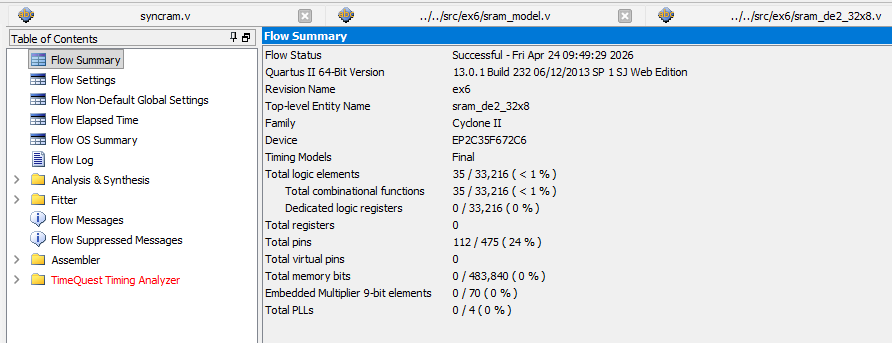
\includegraphics[width=0.9\textwidth]{ex6/complie.png}
    \caption{Biên dịch thành công trên Quartus II}
    \label{fig:ex6_compile}
\end{figure}

\subsubsection{Pin assignment}

Thực hiện gán chân cho toàn bộ các tín hiệu của top-level theo \texttt{DE2\_pin\_assignments.qsf}: \texttt{SW[17:0]}, \texttt{KEY[3:0]}, \texttt{HEX0..HEX7}, \texttt{LEDG[8:0]}, và toàn bộ bus giao tiếp SRAM (\texttt{SRAM\_ADDR[17:0]}, \texttt{SRAM\_DQ[15:0]}, \texttt{SRAM\_CE\_N}, \texttt{SRAM\_OE\_N}, \texttt{SRAM\_WE\_N}, \texttt{SRAM\_UB\_N}, \texttt{SRAM\_LB\_N}).

\begin{figure}[H]
    \centering
    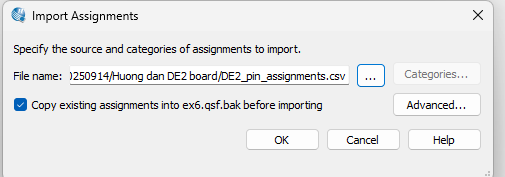
\includegraphics[width=\textwidth]{ex6/pin_assignment.png}
    \caption{Pin Planner sau khi import \texttt{DE2\_pin\_assignments.qsf}}
    \label{fig:ex6_pin}
\end{figure}

\subsubsection{Nạp bit-stream xuống DE2 qua USB-Blaster}

Kết nối board DE2 với PC qua cable USB-Blaster, bật nguồn board ở chế độ RUN, mở \textit{Tools $\rightarrow$ Programmer}, cấu hình Hardware Setup chọn \texttt{USB-Blaster}, thêm file \texttt{.sof} vừa compile và nhấn \textbf{Start} để nạp xuống FPGA.

\begin{figure}[H]
    \centering
    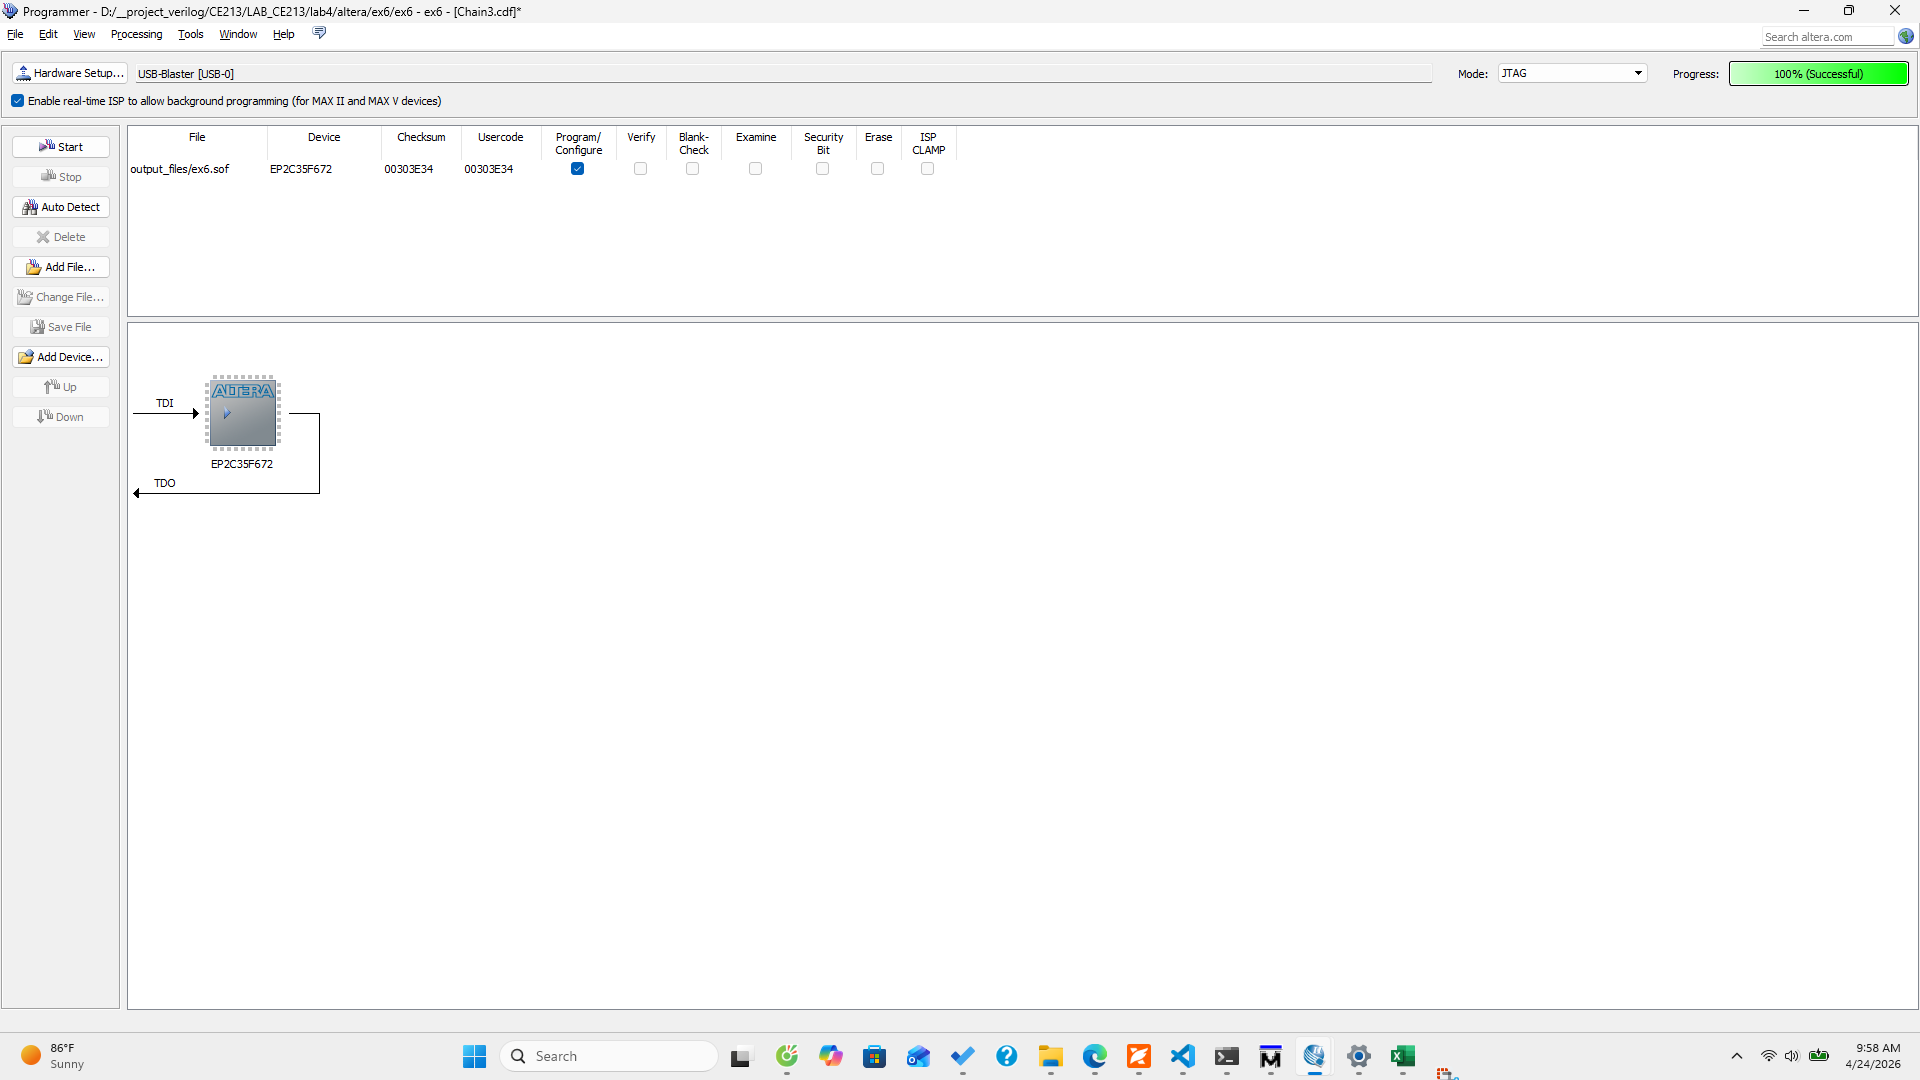
\includegraphics[width=0.9\textwidth]{ex6/load_sof.png}
    \caption{Nạp bit-stream \texttt{.sof} xuống DE2 qua USB-Blaster}
    \label{fig:ex6_load}
\end{figure}

\subsubsection{Kiểm thử đọc/ghi trên board}

Sau khi nạp xong, thực hiện thao tác trên board:
\begin{itemize}[leftmargin=1.5cm]
    \item \textbf{Ghi}: chỉnh \texttt{SW[15:11]} chọn địa chỉ, \texttt{SW[7:0]} đặt dữ liệu, bật \texttt{SW[17]=1} (LEDG[0] sáng báo Write), nhấn \texttt{KEY[0]} để ghi vào SRAM.
    \item \textbf{Đọc}: tắt \texttt{SW[17]=0}, chỉnh \texttt{SW[15:11]} đến địa chỉ cần đọc; giá trị lưu trong SRAM hiển thị ngay trên \texttt{HEX1:HEX0}.
\end{itemize}

\begin{figure}[H]
    \centering
    \begin{subfigure}{0.48\textwidth}
        \centering
        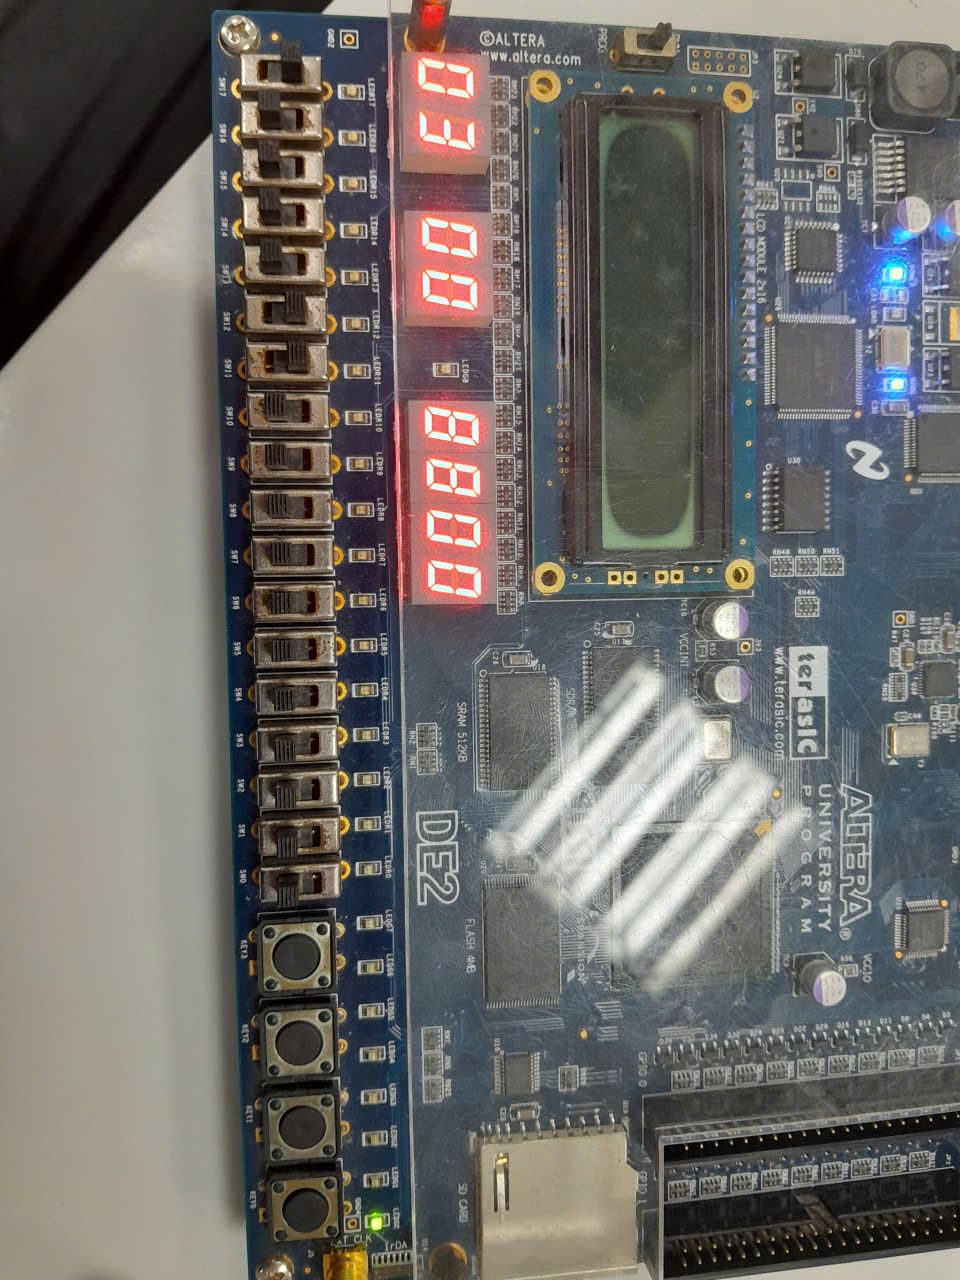
\includegraphics[width=\textwidth]{ex6/de2kit_write.jpg}
        \caption{Thao tác ghi: SW[17]=1, LEDG[0] sáng}
    \end{subfigure}
    \hfill
    \begin{subfigure}{0.48\textwidth}
        \centering
        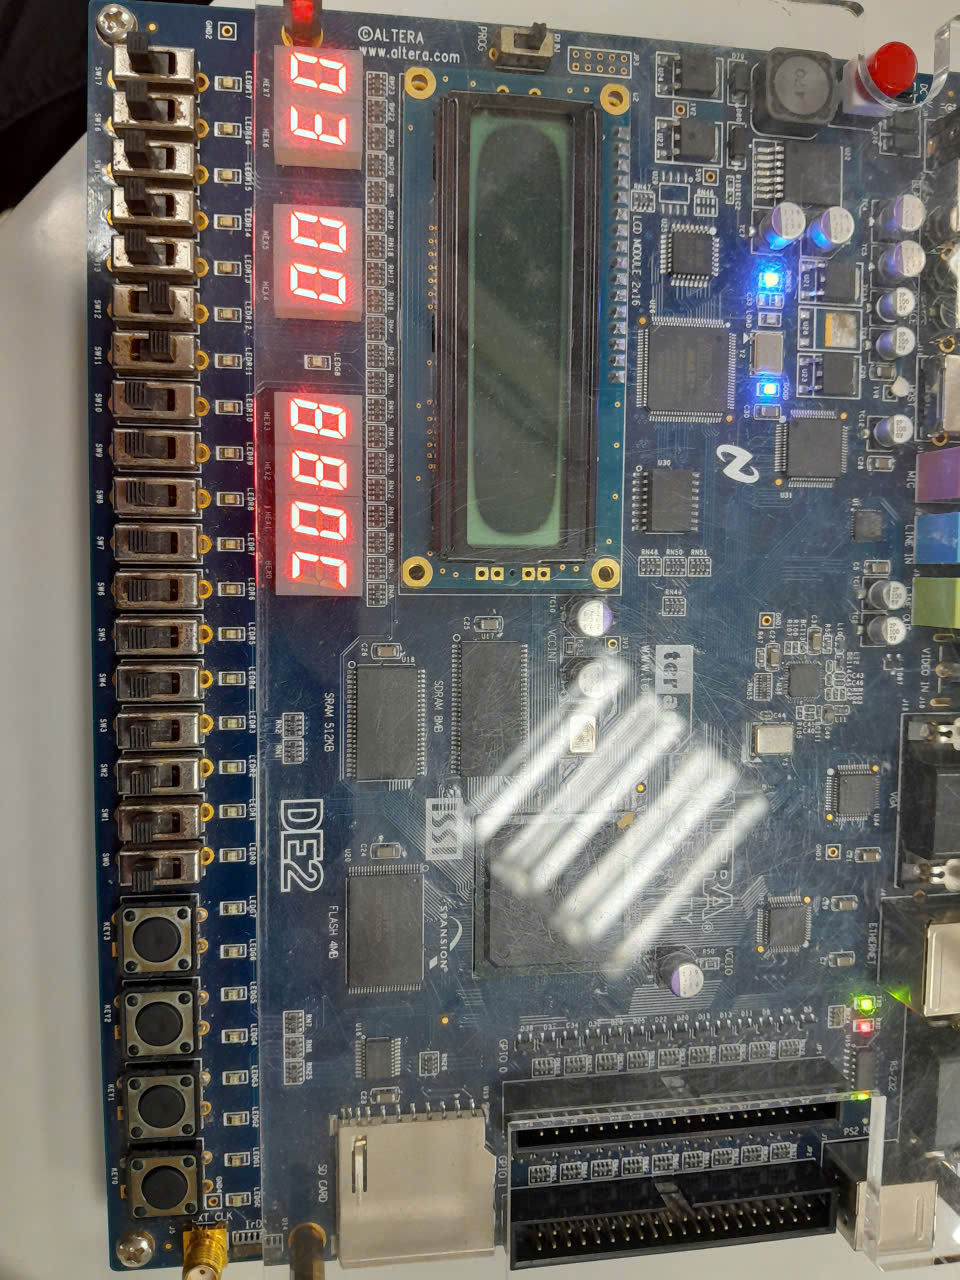
\includegraphics[width=\textwidth]{ex6/de2kit_read.jpg}
        \caption{Thao tác đọc: SW[17]=0, HEX1:HEX0 hiện dữ liệu}
    \end{subfigure}
    \caption{Kiểm thử đọc/ghi SRAM trên board DE2}
    \label{fig:ex6_de2kit}
\end{figure}

\subsubsection{Nhận xét}

\begin{itemize}[leftmargin=1.5cm]
    \item Các cặp (địa chỉ, dữ liệu) ghi vào SRAM đều được đọc lại chính xác trên \texttt{HEX1:HEX0}, khớp với giá trị đã hiển thị trước đó ở \texttt{HEX5:HEX4} (data-in) — phù hợp với kết quả mô phỏng.
    \item Bus inout \texttt{SRAM\_DQ} được xử lý đúng: khi \texttt{SW[17]=1} FPGA drive bus, khi \texttt{SW[17]=0} FPGA thả Z để chip SRAM drive — không xảy ra xung đột bus gây cháy chân I/O.
    \item Việc dùng \texttt{KEY[0]} làm clock ghi (chưa debounce) đôi khi sinh ra nhiều xung do bouncing, nhưng vì mỗi lần nhấn SW/key sau khi đã nhả xong nên chưa thấy lỗi ghi sai. Khi yêu cầu độ ổn định cao hơn có thể thay bằng \texttt{CLOCK\_50} + debouncer.
    \item So với RAM nội \texttt{M4K} (dựng bằng \texttt{MegaWizard / altsyncram}), chip SRAM ngoài cho dung lượng lớn hơn rất nhiều (256K$\times$16), nhưng phải quản lý thêm các chân \texttt{/CE}, \texttt{/OE}, \texttt{/WE}, \texttt{/UB}, \texttt{/LB} và bus inout. Trong phạm vi $32 \times 8$, dùng M4K đơn giản hơn, nhưng thực hành với SRAM ngoài giúp hiểu rõ giao thức bus bất đồng bộ và cách xử lý tri-state trên FPGA.
\end{itemize}

\newpage

% ============================================================================
%  PHỤ LỤC - README
% ============================================================================
\section{Phụ lục -- Nội dung \texttt{README.md}}

File \texttt{lab4/README.md} tóm tắt cách tổ chức dự án, cách chạy mô phỏng và hướng dẫn chi tiết cho Ex6 (SRAM DE2). Nội dung đầy đủ xem trong repository; phần dưới đây trích các mục chính:

\begin{lstlisting}[style=md, caption={Trích lược \texttt{lab4/README.md}}]
# Lab 4 - Kiem tra thiet ke su dung Testbench

## Cach chay mo phong trong ModelSim-Altera

cd D:/__project_verilog/CE213/LAB_CE213/lab4/src/exN
vlib work
vlog <dut>.v <tb>.v
vsim -voptargs=+acc work.<tb>
add wave -r *
run -all

## Bang cac testbench

| Bai  | File DUT                   | Testbench                   | Loai          |
|------|---------------------------|-----------------------------|---------------|
| 1    | ex1/alu32.v               | tb_alu32.v                  | self + $monitor |
| 2.1  | ex2/counter4.v            | tb_counter4_wave.v          | wave          |
| 2.2  | ex2/counter4.v            | tb_counter4_self.v          | self-checking |
| 3    | ex3/reg_file_32x32.v      | tb_reg_file_32x32.v         | self-checking |
| 4    | ex4/dual_port_ram_1kx8.v  | tb_dual_port_ram_1kx8.v     | self-checking |
| 5.1  | ex5/sp_ram_128x8.v        | tb_sp_ram_128x8_wave.v      | wave          |
| 5.2  | ex5/sp_ram_128x8.v        | tb_sp_ram_128x8_self.v      | self-checking |
| 6    | ex6/sram_de2_32x8.v       | tb_sram_de2_32x8.v          | self + sram_model |

Tieu chi PASS: cuoi log co dong RESULT : ALL TESTS PASSED va fail=0 trong
dong SUMMARY.

## Bai 6 - Huong dan SRAM DE2

  1. Dac diem chip IS61LV25616AL-10 (256K x 16-bit)
  2. Bang pin DE2 <-> SRAM (SRAM_ADDR, SRAM_DQ, SRAM_CE_N, ...)
  3. Timing chinh (tAA <= 10ns, tAW >= 8ns, tSD >= 6ns)
  4. Cac buoc Quartus II + DE2:
       - Tao project target Cyclone II EP2C35F672C6
       - Viet top-level sram_de2_32x8.v voi inout SRAM_DQ
       - Pin assignment bang DE2_pin_assignments.qsf
       - Compile -> download .sof qua USB-Blaster
       - Kiem thu: chinh SW, nhan KEY, quan sat HEX0..HEX1
  5. Cach thay the: dung MegaWizard (RAM: 1-PORT) tao ramlpm.v,
     them Allow In-System Memory Content Editor de xem qua JTAG.
\end{lstlisting}

\newpage

% ============================================================================
%  KẾT LUẬN
% ============================================================================
\section{Kết luận}

Qua Lab 4, nhóm đã thực hành thiết kế, viết testbench và kiểm tra 6 bài tập bằng ModelSim-Altera:

\begin{enumerate}
    \item \textbf{ALU 32-bit} (8 op-code): testbench kết hợp \texttt{\$display}/\texttt{\$monitor} và self-check. Kết quả: \textbf{32/32 PASS}.
    \item \textbf{Counter 4-bit} (async reset, enable, up/down): 2 testbench (wave + self-check). Kết quả: \textbf{62/62 PASS}.
    \item \textbf{Register File 32$\times$32} (2 read ports, 1 write port, sync write / async read): self-checking. Kết quả: \textbf{170/170 PASS}.
    \item \textbf{Dual-port RAM 1024$\times$8} (1R1W sync, gated read/write): self-checking. Kết quả: \textbf{362/362 PASS}.
    \item \textbf{Single-port Sync RAM 128$\times$8, bus inout}: 2 testbench (wave + self-check). Kết quả: \textbf{183/183 PASS}.
    \item \textbf{External SRAM DE2} (\texttt{IS61LV25616AL-10}): top-level $32 \times 8$ + behavioral model + testbench. Kết quả mô phỏng: \textbf{34/34 PASS}. Đã nạp bit-stream xuống board DE2, thao tác ghi/đọc SRAM qua SW/KEY và quan sát \texttt{HEX1:HEX0} hoạt động đúng như mô phỏng.
\end{enumerate}

Các kỹ thuật chính đã áp dụng:
\begin{itemize}
    \item \textbf{Self-checking testbench}: duy trì golden model song song với DUT, so sánh từng cycle và đếm pass/fail.
    \item \textbf{Dual logging}: in ra stdout + file \texttt{.log} kèm timestamp để dễ kiểm tra lại.
    \item \textbf{Watchdog timeout}: chặn simulation vô hạn.
    \item \textbf{Random stimulus}: dùng \texttt{\$random} để tăng coverage sau các test case định hướng.
    \item \textbf{Xử lý bus inout}: dùng cặp \texttt{reg drv\_data} + \texttt{assign tri-state} để bên TB drive hoặc thả Z, tránh xung đột với DUT.
    \item \textbf{Behavioral model chip ngoài}: viết \texttt{sram\_model.v} mô phỏng chip \texttt{IS61LV25616AL} để kiểm tra top-level trước khi nạp xuống board.
\end{itemize}

Tổng cộng \textbf{843/843 check PASS} trên toàn bộ Lab 4.

\end{document}
